\documentclass{scrartcl}
%\usepackage[latin1]{inputenc}
\usepackage{amsmath}
\usepackage[ngerman]{babel}
\usepackage{amsfonts}
\usepackage{amssymb}
%\usepackage{amstext}
%\usepackage{csquotes}
%\usepackage{parskip}
%\usepackage{esdiff}
\usepackage{graphicx}
\usepackage{figsize}
\usepackage{float}
\usepackage{geometry}
\geometry{verbose,tmargin=2.5cm,bmargin=2.5cm,lmargin=2.5cm,rmargin=2.5cm}
%\usepackage{graphics} %Origin Grapheneinbundung
%\usepackage{wrapfig}
%\usepackage{textcomp}
%\usepackage{epstopdf}
%\usepackage{setspace}
%\usepackage{trfsigns}
%\usepackage{verbatim}
\usepackage[format=plain,font=small,labelfont=bf]{caption}
\usepackage[OT2,T1]{fontenc}
\DeclareSymbolFont{cyrletters}{OT2}{wncyr}{m}{n}
\DeclareMathSymbol{\Sha}{\mathalpha}{cyrletters}{"58}
\selectlanguage{ngerman}
\begin{document}


%\begin{titlepage}
%	\title{Praktikum B - Versuch B3.4: Positronen - Emissions - Tomografie}
%	\author{Jesco Talies, Timon Danowski, Erik Ga"smus}
%	\maketitle
%	\center
%	\textbf{Versuchsdatum: 07.12.2020}
%\end{titlepage}
%\thispagestyle{empty}

%\setcounter{page}{0}



\thispagestyle{empty}
\vspace*{\fill}
\begin{center}
	\Huge
	\textbf{Universit"at zu K"oln}\\
	\LARGE
	\textbf{Institut f"ur Kernphysik}\\
	\vspace{2cm}
	\textbf{Versuchsprotokoll}\\
	\vspace{0.5cm}
	\large
	\textbf{B3.2: $\gamma$-Spektroskopie mit einem HPGe-Detektor}\\
	\normalsize
	\vspace{2cm}
	\begin{tabular}{r l}
		Autoren: 	& Jesco Talies$^1$\\
					& Timon Danowski$^2$\\
					& Erik Ga"smus$^3$\\\\
		Durchgefuehrt am:	& 30.11.2020\\
		Betreuer:	& Miriam M"uscher
	\end{tabular}
\end{center}
\vfill\footnotesize
$^1$ jtalies@smail.uni-koeln.de, Matrikel-Nr.: 7348338\\
$^2$ tdanowsk@smail.uni-koeln.de, Matrikel-Nr.: 7348629\\
$^3$ e.gassmus@gmail.com, Matrikel-Nr.: 7329899
\normalsize

\newpage
\thispagestyle{empty}
\tableofcontents
\clearpage
\setcounter{page}{1}





\section{Einleitung}

In der Kernphysik interessiert man sich, wie der Name bereits sagt, f"ur Vorg"ange innerhalb der Atomkerne. Diese sind der direkten Beobachtung nicht zug"anglich, wir kennen jedoch einige Effekte, wie z.B. den Radioaktiven Zerfall, durch die wir R"uckschl"usse auf derartige Vorg"ange gewinnen k"onnen. In diesem Versuch untersuchen wir die $\gamma$ - Strahlung, die Kerne emittieren, wenn sie sich nach einem $\beta$ - Zerfall in einem angeregten Zustand befinden und kurz darauf in einen energetisch g"unstigeren Zustand "ubergehen. Dabei interessieren wir uns besonders f"ur die Funktionsweise des dabei verwendeten High Purity Germanium - Detektors (kurz: HPGe) und welche weiteren Informationen "uber die Wechselwirkung von $\gamma$ - Quanten mit Materie wir aus den aufgenommenen Spektren gewinnen k"onnen.

\section{Theoretische Grundlagen}

\subsection{Atomkerne}

Zun"achst m"ochten wir uns ein Bild davon machen, wie die im Versuch beobachtete Strahlung zustande kommt, wozu wir kurz einige Aspekte der Kernphysik wiederholen. "Ahnlich wie die Elektronen in der Atomh"ulle werden die Atomkerne als Quantenobjekte durch entsprechende Quantenzahlen charakterisiert: Die Kernladungszahl Z gibt die Protonenzahl an, die Massenzahl A die Summe aus Protonen- und Neutronenanzahl. Zum Verst"andnis der Kern"uberg"ange sind zudem die Parit"atsquantenzahl $\pi$ des Kerns (also sein Verhalten unter Raumspiegelung) sowie seine Gesamtdrehimpuls- oder Kernspinquantenzahl $\vec{I} = \sum_{i=1}^{A}(\vec{s}_{i} + \vec{l}_{i}$) wichtig.\\
Im Grundzustand nehmen alle Kernbausteine den energetisch niedrigstm"oglichen Zustand an. Dazu bilden Protonen und Neutronen jeweils untereinander Paare mit antiparallel ausgerichteten Spins (das Tr"opfchenmodell ber"ucksichtigt dies z.B. im Paarungsterm). Im Gesamtkernspin heben sich diese antiparallel ausgerichteten Spins genau weg (vgl. Spinquantenzahlformel oben), sodass Kerne mit sowohl gerader Protonen- als auch Neutronenzahl im Grundzustand Spin 0 haben. In angeregten Zust�nden solcher Kerne verbleibt dann im Gesamtspin ein Paar (oder mehrere) parallel ausgerichteter Spins, die sich jeweils zu einem ganzzahligen Gesamtspin addieren. Ist entweder die Protonen- oder Neutronenzahl des Kerns ungerade und die verbleibende Teilchenzahl gerade (gu bzw. ug - Kerne), bleibt immer mindestens ein Kernteilchen ohne Partner, das seinen Spin durch antiparallele Ausrichtung kompensieren k"onnte. Die Spinquantenzahl ist im Grundzustand also mindestens $1/2$ (z.B. bei  $^1_1$H) und immer halbzahlig (z.B. $9/2$ f"ur $^{209}_{83}$Bi). Liegen Protonen und Neutronen in ungerader Anzahl vor, k"onnen zwar prinzipiell alle Spins sich zu 0 kompensieren (z.B. bei $^{206}_{81}$Tl), es k"onnen jedoch auch h"ohere, stets ganzzahlige Werte auftreten (z.B. 1 f"ur $^{14}_{7}$N).\\
%: Bei ug oder gu - Kernen (gerade bzw ungerade in Bezug auf Protonen- und Neutronenzahl) ist dieser Wert halbzahlig (z.B. $1/2$ f"ur $^1_1$H oder $9/2$ f"ur $^{209}_{83}$Bi), bei gg - Kernen 0 (und ganzzahlig in angeregten Zust"anden) und bei uu - Kernen ist er zwar ganzzahlig, kann jedoch auch im Grundzustand gr"o"ser sein als 0 (z.B. 0 f"ur $^{206}_{81}$Tl, aber 1 f"ur $^{14}_{7}$N).\\
Liegt ein Kern nun beispielsweise nach einem $\beta$ - Zerfall in einem angeregten Zustand vor, kann er unter Ber"ucksichtigung einiger im Folgenden besprochenen Auswahlregeln in einen energetisch niedrigeren Zustand "ubergehen. Die Energie der dabei emittierten Strahlung entspricht der Differenz der Energien des jeweiligen Anfangs- und Endzustands des Kerns:

\begin{equation}
E_{\gamma} = E_i -  E_f
\end{equation}

Bei diesem Vorgang handelt es sich um einen Zweik"orperzerfall, Energie und Impuls m"ussen also erhalten sein. Es tritt also ein R"ucksto"s auf den Kern auf, da dieser den Impuls $p = E_{\gamma}/c$ des $\gamma$ - Quants mit seinem Impuls $P = -p$ (im Ruhesystem des Kerns) kompensieren muss. Aus der Energieerhaltung ergibt sich f"ur die vom Kern aufgenommene Enrgie in klassischer N"aherung

\begin{equation}
E_{\text{R"ucksto"s}} = \frac{P^2}{2M} = \frac{E_{\gamma}^2}{2Mc^2}
\end{equation}


Die Multipolarit"at des "Ubergangs und ebenso der dabei emittierten Strahlung ergibt sich aus der Drehimpulsdifferenz des Anfangs- und Endzustandes. Man unterscheidet zwischen elektrischer und magnetischer Multipolstrahlung und bezeichnet diese mit $E\ell$ bzw. $M\ell$, wobei $\ell$ f"ur die jeweilige Multipolarit"at, also den Drehimpuls der Strahlung (in Einheiten von $\hbar$) steht; $E1$ bezeichnet also elektrische Dipolstrahlung, $M2$ bezeichnet magnetische Quadrupolstrahlung usw.. Elektrische und magnetische Multipol"uberg"ange der gleichen Ordnung haben den gleichen Drehimpuls $\ell$, aber entgegengesetzte Parit"at: $E\ell$ - Strahlung hat Parit"at $+(-1)^{\ell}$, $M\ell$ - Strahlung hat Parit"at $-(-1)^{\ell}$. \\
Welche Strahlungsart bei einem "Ubergang entsteht, ist abh"angig von der damit einhergehenden Drehimpuls"anderung im Kern; die Drehimpulsdifferenz zwischen den zwei Kernzust"anden wird von der Strahlung weggetragen, sodass die Drehimpulserhaltung insgesamt erf"ullt ist. Die Drehimpulserhaltung bedingt auch die Auswahlregeln, welche sich aus Fermis goldener Regel ergeben: Bezeichnen $|E^{(0)}_i \rangle$ und $|E^{(0)}_f \rangle$ zwei L"osungen der Zeitunabh"angigen Schr"odingergleichung des Kerns, und wir m"ochten wissen, mit welcher Wahrscheinlichkeit ein "Ubergang zwischen diesen Zust"anden stattfindet, so m"ussen wir das "Ubergangsmatrixelement mithilfe des St"oroperators $H_1$ berechnen:

\begin{equation}
|\langle E^{(0)}_f | H_1 | E^{(0)}_i \rangle |
\end{equation}

Ist dieses Matrixelement Null, so handelt es sich um einen verbotenen "Ubergang, der nur mit sehr niedriger Wahrscheinlichkeit stattfinden kann. Aus der Orthogonalit"at der Zust"ande folgt, dass somit bevorzugt "Uberg"ange stattfinden, bei denen die Regeln
	\\
		$|I_i - I_f| \leq \ell \leq I_i + I_f$\\
		$\pi_i \cdot \pi_f = (-1)^{\ell}$ f"ur $E\ell$\\
		$\pi_i \cdot \pi_f = -(-1)^{\ell}$ f"ur $M\ell$\\
	\\
erf"ullt sind.\\
Die Strahlungsenergien, die durch diese Prozesse erreicht werden, variieren von ca. 100 keV bishin zu 10 MeV. Das m"ogliche $\gamma$ - Spektrum "uberschneidet sich also auch mit dem R"ontgenspektrum. Man unterscheidet diese nicht aufgrund der Energie, sondern wegen des Enstehungsprozesses: $\gamma$ - Strahlung entsteht bei Kernreaktionen, R"ontgenstrahlung bei der Abbremsung oder Ablenkung geladener Teilchen mit hoher kinetischer Energie (i.d.R. Elektronen, Bremsstrahlung) oder bei hochenergetischen "Uberg"angen von H"ullenelektronen im Atom.



\subsection{Wechselwirkung von $\gamma$ - Strahlung mit Materie}

Bei Interaktionen einzelner Teilchen miteinander handelt es sich bekanntlich nicht um deterministische,
 sondern statistische Vorgänge. Wenn wir wissen möchten, mit welcher Wahrscheinlichkeit ein solcher
 Wechselwirkungsvorgang im Einzelfall eintritt, gibt uns der zugehörige Wirkungsquerschnitt $\sigma$ auskunft.
Anschaulich ist der Wirkungsquerschnitt als effektive Trefferfläche der Teilchen im Target eines Stoßprozesses
 zu verstehen. In der Kernphysik gibt man ihn in der Einheit Barn an ( $1b = 10^{-28}m^2 = 100 fm^2 $ ).\\
Man unterscheidet drei grundlegende Arten der Wechselwirkung von $\gamma$ - Strahlung mit Materie:

	\begin{itemize}
		\item{Photoeffekt}
		\item{Compton - Streuung}
		\item{Paarerzeugung}
	\end{itemize}

Diese fassen wir im Folgenden kurz zusammen.


\paragraph{Photoeffekt}

Wenn ein $\gamma$ - Quant auf ein Atom trifft, kann es seine Energie an eines der H"ullenelektronen abgeben, indem es von diesem Elektron absorbiert wird. Ionisierungsenergien liegen meist im eV - Bereich, sodass das Elektron durch die Energieaufnahme aus der Atomh"ulle befreit wird. Seine kinetische Energie ist danach gleich der Energie des absorbierten $\gamma$ - Quants abz"uglich der Bindungsenergie; da Letztere jedoch um ein Vielfaches kleiner ist, vernachl"assigen wir diese in folgenden Betrachtungen und sehen die Energie eines solchen Photo - Elektrons als dieselbe Energie des urspr"unglichen Photons an.\\
Der Wirkungsquerschnitt des Photoeffekts ist abh"angig von der Kernladungszahl $Z$ des getroffenen Atoms sowie der Photonenenergie $E_{\gamma}$:

	\begin{equation}
		\sigma \propto Z^5 E^{-3,5}_{\gamma}
	\end{equation}

Bei Photonenenergien bis ca. 100 keV ist der Photoeffekt der am H"aufigsten eintretende Wechselwirkungsprozess zwischen $\gamma$ - Quanten und Materie.


\paragraph{Comtpon - Streuung}

Freie Elektronen k"onnen anders als ihre in Atomen gebundenen Artgenossen nicht die gesamte Energie eines $\gamma$ - Quants aufnehmen, es gibt stattdessen ein Kontinuum m"oglicher Werte f"ur die "ubertragene Energie, bestimmt durch die Klein - Nishina - Formel. Die "ubertragene Energie legt den Streuwinkel $\theta$ fest, mit welchem f"ur die "Anderung der Wellenl"ange des Photons
% Wie viel Energie sie bei einem Sto"s erhalten, ist abh"angig vom Streuwinkel $\theta$. Der Energie"ubertrag auf das Elektron wird maximal f"ur $180^{\circ}$, also R"uckstreuung des Photons, und ist 0 bei $\theta = 0$. Die "Anderung der Wellenl"ange (und damit der Energie) des Photons beim Sto"s ergibt sich aus der Klein - Nishina Formel zu

	\begin{equation}
		\Delta \lambda = \frac{h}{m_{e}c}(1-\cos{\theta})
		\label{eq:com}
	\end{equation}


gilt. Ein maximaler Energie"ubertrag bedingt einen Streuwinkel von $180^{\circ}$, also eine exakte R"uckstreuung, und wenn keine Energie "ubertragen wird, tritt auch keine Streuung auf ($\theta = 0$).

F"ur den Wirkungsquerschnitt der Compton - Streuung gilt

	\begin{equation}
		\sigma \propto ZE^{-1}_{\gamma}
	\end{equation}

Ab Photonenenergien von ca. 100 keV wird die Compton - Streuung zur dominierenden Wechselwirkungsform.


\paragraph{Paarerzeugung}

Elektronen und Positronen haben eine Ruhemasse von jeweils 511 keV. Ab einer Photonenenergie von 1022 keV kann es also zur Paarerzeugung kommen, d.h. das $\gamma$ - Quant kann in ein Elektron - Positron - Paar zerfallen. Notwendige Bedingung f"ur diesen Prozess ist neben der genannten Mindestenergie die Anwesenheit eines Atomkerns, der durch Aufnahme des Photonenimpulses als R"ucksto"s die Impulserhaltung gew"ahrleistet. "Ubersteigt die Energie des $\gamma$ - Quants 1022 keV, erhalten die entstehenden Leptonen diese "ubersch"ussige Energie als kinetische Energie.\\
Der Wirkungsquerschnitt der Paarerzeugung nimmt mit der Photonenenergie zu,

	\begin{equation}
		\sigma \propto Z^2 \ln{E_{\gamma}}
	\end{equation}

sodass ab Energien von wenigen MeV (abh"angig von der Kernladungszahl $Z$) die Paarerzeugung den Hauptanteil der Wechselwirkungen zwischen $\gamma$ - Strahlung und Materie ausmacht.


\subsubsection{Das $\gamma$ - Spektrum}

\begin{figure}[!ht]
	\centering
	\SetFigLayout{1}{1}
	\includegraphics[width=350px, totalheight=350px, keepaspectratio]{gammaspektrumanleitung.PNG}
	\caption{Bsp. eines $\gamma$ - Spektrums mit zwei unterschiedlichen "Ubergangsenergien (Quelle: Praktikumsanleitung)}
	\label{figspektrum}
\end{figure}

Unter Kenntnis dieser Grundlegenden Wechselwirkungsarten k"onnen wir nun erkl"aren, wie ein typisches $\gamma$ - Spektrum, wie es in Abb. \ref{figspektrum} f"ur eine Quelle mit zwei Kern"uberg"angen unterschiedlicher Energien gezeigt ist, zustande kommt.\\
Die gro"sen, mit 1 und 2 markierten Peaks werden als Full - Energy - Peak bezeichnet. Sie entstehen, wenn die gesamte Energie des Photons im Detektor deponiert wird und geben somit auskunft "uber die frei werdende Energie bei den einzelnen
 "Uberg"angen. Marker 5 und 6 geh"oren zu den Compton - Kanten, jeweils eine zu jedem "Ubergang. Diese kommen durch Elektronen zustande, an denen die $\gamma$ - Quanten Compton - gestreut werden. Die Kante bildet sich dadurch aus, dass bei der Compton - Streuung
 niemals die volle Energie des Photons an ein Elektron abgegeben werden kann, der maximal "ubertragene Energieanteil ist durch Formel \ref{eq:com} bestimmt und ergibt sich, in Abh"angigkeit von der Frequenz $\nu$ des einfallenden Photons, f"ur einen Streuwinkel von $180^{\circ}$ zu

	\begin{equation}
	E_{e^-}|_{\theta = \pi} = \frac{2h\nu / m_0 c^2}{1+2h\nu /m_0 c^2} = \frac{E_{\gamma}}{1 + \frac{511\text{keV}}{2E_{\gamma}}}
	\label{eqCK}
	\end{equation}

wobei $m_0$ die Ruhemasse des Elektrons bezeichnet (die mit dem Faktor $c^2$ verrechnet 511keV ergibt). Diesem Wert entspricht die Position der Compton - Kante.\\
 Bei einem Winkel von $\theta = 0$ wird gar keine Energie auf das Elektron "ubertragen, und f"ur beliebige Winkel zwischen 0 und $180^{\circ}$ gilt

	\begin{equation}
	E_{e^-} = h\nu (\frac{(h\nu / m_0 c^2)(1 - \cos{\theta})}{1 + (h\nu / m_0 c^2)(1 - \cos{\theta})})
	\end{equation}

wodurch sich jeweils links von den Compton - Kanten das dazugeh"orige Compton - Kontinuum bildet (sh. Abb. \ref{comptinuum}).


\begin{figure}[!ht]
	\centering
	\SetFigLayout{1}{1}
	\includegraphics[width=350px, totalheight=350px, keepaspectratio]{comptinuum.PNG}
	\caption{Auswirkungen des Compton - Effekts auf das Spektrum (Quelle: Knoll: \textit{Radiation Detection and Measurement}, Wiley, 2000)}
	\label{comptinuum}
\end{figure}



 Es kann vorkommen, dass ein $\gamma$ - Quant in unmittelbarer Detektorn"ahe au"serhalb des Detektors Compton - gestreut wird (z.B. am K"uhlfinger, sh. Detektoraufbau in Abschnitt 2.3) und mit seiner dadurch reduzierten Energie anschlie"send im Detektor registriert wird. Dieser Effekt bedingt den mit 7 markierte R"uckstreupeak.\\
Die mit 3, 4 und 8 markierten Peaks sind Folgen der Paarerzeugung. Das bei der Paarerzeugung entstehende Positron wird nach kurzer Zeit seine kinetische Energie durch St"o"se abgeben, bis es nur noch in etwa thermische Energie hat und anschlie"send mit einem Elektron unter kollinearer Emission zweier 511 keV - Photonen annihilieren. Wenn beide Photonen ihre Energie im Detektor abgeben, summiert sich die im Detektor deponierte Energie zum Full - Energy - Peak auf. Entkommt jedoch eines oder sogar beide der bei der Annihilation entstehenden Photonen aus dem Detektor ohne zu wechselwirken, so liegt die im Detektor deponierte Energie 511 keV (Single - Escape - Peak, Marker 3) bzw 1022 keV (Double - Escape - Peak, Marker 4) darunter.\\
Marker 8 zeigt einen weiteren Peak bei 511 keV, der entsteht, wenn die Paarerzeugung au"serhalb des Detektors stattfindet und eines der bei der darauf folgenden Annihilation emittierten Photonen im Detektor erfasst wird.



\subsubsection{Das Absorptionsgesetz}

Ein Absorber der Dicke $d$ und Fl"ache $A$ zwischen Quelle und Detektor hat eine Abschw"achung der Strahlungsintensit"at zur Folge. Mit $I_0$, der Intensit"at ohne Absorber, ergibt sich f"ur die Intensit"at das Lambert - Beer - Gesetz:

\begin{equation}
I(d) = I_0 \cdot e^{-\mu d},
\end{equation}

mit dem linearen Abschw"achungskoeffizienten $\mu$. Dieser ist eine Materialkonstante (Einheit: cm$^{-1}$), die sich aus der Wahrscheinlichkeit daf"ur, dass ein $\gamma$ - Quant innerhalb des Absorbers wechselwirkt, ergibt. Das Absorptionsgesetz l"asst sich dementsprechend auch "uber den Wirkungsquerschnitt $\sigma$ des Absorbermaterials ausdr"ucken. Betrachten wir $\sigma$ als Zusammengesetzt aus den Wirkungsquerschnitten f"ur Photoeffekt, Comptonstreuung und Paarerzeugung, $\sigma = \sigma_{\text{Photo}} + \sigma_{\text{Compton}} + \sigma_{\text{Paar}}$ und bezeichnen mit $n$ die Teilchenkonzentration des Absorbers, so ist $n\sigma$ die Wahrscheinlichkeit daf"ur, dass ein $\gamma$ - Quant beim Durchqueren des Absorbers absorbiert wird, und es gilt ebenso

\begin{equation}
I(d) = I_0 \cdot e^{-n\sigma d},
\end{equation}



\subsection{Der Halbleiterdetektor}

Das B"andermodell erkl"art die Leitf"ahigkeit eines Materials dadurch, dass Elektronen,
 wenn sie das Leitungsband eines Materials besetzen, zum elektrischen Strom beitragen k"onnen.
  Je nach Material ist das Leitungsband immer teilweise besetzt, nur bei thermischer Anregung (oder anderweitiger Energiezufuhr), oder fast nie. Der energetisch h"ochste Zustand, der in einem Material bei einer Temperatur von 0 Kelvin noch mit Elektronen besetzt ist, kennzeichnet die Fermi - Energie des Materials. Liegt diese im Leitungsband, handelt es sich um einen elektrischen Leiter. Liegt die Fermi - Energie unterhalb des Leitungsbandes, so handelt es sich entweder um einen Halbleiter oder einen Isolator, welche man Anhand der gr"o"se der Bandl"ucke, die Elektronen "uberwinden m"ussen, um ins Leitungsband zu gelangen, unterscheidet: Bei einer Bandl"ucke von ca. 0,1 bis 4 eV spricht man von einem Halbleiter, bei gr"o"seren Bandl"ucken von Isolatoren. \\
Im Halbleiter k"onnen Elektronen die Energie zur "uberwindung der Bandl"ucke von Phononen erhalten, was durch Gitterfehler im Kristall beg"unstigt werden kann und die intrinsische Leitf"ahigkeit halbleitender Materialien bedingt. Die Wahrscheinlichkeit zur Ausbildung derartiger Gitterfehler nimmt mit der Temperatur zu, da sie die Entropie des Gitters erh"ohen und somit themodynamisch beg"unstigt sind. Durch K"uhlung l"asst sich dieser Effekt sowie die Anregung durch Phononen und somit die intrinsische Leitf"ahigkeit insgesamt unterdr"ucken.\\
\\
Die Leitf"ahigkeit eines Halbleiters l"asst sich durch das Einbringen von Fremdatomen ins Kristallgitter kontrolliert manipulieren. Bringt man ein Fremdatom ein, dass im Gegensatz zum restlichen Gitter weniger Valenzelektronen zur Verf"ugung hat, spricht man von p - Dotierung; die Fremdatome dienen in diesem Fall als Elektronenakzeptoren und im B"andermodell entsteht dadurch ein zus"atzliches diskretes Energieniveau knapp oberhalb des Valenzbandes. Das einbringen eines Fremdatomes, das im Vergleich zum Gitter zus"atzliche Valenzelektronen hat, wird als n - Dotierung bezeichnet. Ein solches Fremdatom dient als Elektronendonator und bedingt im B"andermodell ebenfalls ein zus"atzliches diskretes Energieniveau zwischen Leitungs- und Valenzband (jedoch im Vergleich zur p - Dotierung n"aher am Leitungsband).\\
\\
Beim Zusammenf"uhren einer p - und einer n - Dotierten Schicht entsteht ein pn - "Ubergang, in welchem die Elektronen der Donatoren der n - Schicht in die p - Schicht diffundieren und dort mit den Akzeptoren rekombinieren k"onnen (analog geben die Akzeptoren L"ocher an die Donatoren ab).
% Dadurch entsteht eine Raumladungs- bzw. Verarmungszone, die die Leitf"ahigkeit des Materials unterdr"uckt.
Die zuvor elektrisch neutralen Akzeptoren und Donatoren weisen infolge dieser Elektronen- und L"ocherdiffusion nun "ubersch"ussige negative bzw positive Ladungen auf, wodurch sich ein elektrisches Feld zwischen beiden Schichten aufbaut, das der Diffusion entgegenwirkt, bis sich ein Gleichgewicht zwischen beiden Effekten einstellt. Das verbleibende elektrische Feld bewegt die freien Ladungstr"ager im Bereich des pn - "Ubergangs aus diesem heraus, wodurch sich dort schlie"slich die sogenannte \textit{Raumladungszone} oder auch \textit{Verarmungszone} ausbildet.
Durch das Anlegen einer "au"seren Spannung $U$ kann die Ausdehnung dieses Bereichs variiert werden. Je nachdem, in welche Richtung die Spannung angelegt wird, wird die Verarmungszone vergr"o"sert oder abgebaut; den ersten Fall bezeichnet man als Sperrrichtung, da ein Stromfluss dadurch noch weiter unterdr"uckt wird, den zweiten Fall als Durchlassrichtung, da ein Abbau der Verarmungszone einen Stromfluss erm"oglicht. F"ur die Ausdehnung $d$ der Verarmungszone gilt:

\begin{equation}
	d \approx \sqrt{\frac{2\epsilon_0 \cdot U}{e \cdot N}}
	\label{verarmungszone}
\end{equation}

$N$ bezeichnet die Verunreinigungskonzentration, die meist im Bereich von 0,1 bis 100 ppm liegt. Wenn man die Raumladungszone maximieren will, wird ersichtlich, dass dazu zum einen eine hohe Spannung sowie eine niedrige Verunreinigungskonzentration n"otig sind. Wir wollen dies deshalb erreichen, da uns die Raumladungszone als Detektionsvolumen dient: der in Sperrrichtung betriebene pn - "Ubergang verhindert einen Stromfluss, wenn jedoch ein $\gamma$ - Quant innerhalb der Raumladungszone wechselwirkt und somit Energie an die dortigen Elektronen "ubertr"agt, k"onnen diese dennoch ins Leitungsband gelangen. $\gamma$ - Quanten, die in der Verarmungszone wechselwirken, erzeugen also einen geringen Stromfluss.\\
Da wir m"oglichst viele der von einer radioaktiven Quelle emittierten $\gamma$ - Quanten registrieren wollen, ist es w"unscheswert, das effektive Detektionsvolumen zu erh"ohen. Neben dem Betrieb des Detektors in Sperrrichtung kann eine geeignete Wahl der Detektorgeometrie dies weiter beg"unstigen, weshalb der verwendete Detektor eine koaxiale Geometrie hat. In Abb. \ref{figdetektorvert} ist eine m"ogliche Umsetzung eines solchen Detektors im vertikalen Querschnitt dargestellt, Abb. \ref{figdetektorhoriz} zeigt einen entsprechenden horizontalen Querschnitt.

\begin{figure}[!ht]
	\centering
	\SetFigLayout{1}{1}
	\includegraphics[width=250px, totalheight=250px, keepaspectratio]{coaxialdetector.jpg}
	\caption{Vertikaler Detektorquerschnitt\\ (Quelle: http://www.canberra.com/fr/produits/detectors/germanium-detectors.asp)}
	\label{figdetektorvert}
\end{figure}


\begin{figure}[!ht]
	\centering
	\SetFigLayout{1}{1}
	\includegraphics[width=250px, totalheight=250px, keepaspectratio]{dotierungkoaxialgeometrie.jpg}
	\caption{Horizontaler Detektorquerschnitt\\ (Quelle: https://docplayer.org/docs-images/81/83374154/images/34-0.jpg)}
	\label{figdetektorhoriz}
\end{figure}


Das durch das wandern der Ladungstr"ager in Richtung p - bzw. n - Schicht entstehende elektrische Feld l"asst sich analog zu dem eines Kondensators mit entsprechender Geometrie verstehen. F"ur die Kapazit"at eines planaren Kondensators mit Plattenabstand $d$ und Plattenfl"ache $A$ beispielsweise gilt $C = \epsilon \epsilon_0 A / d$. Betrachten wir $d$ gem"a"s Gl. \ref{verarmungszone} als Ausdehnung der Verarmungszone, wird die Verbindung zur Kapazit"at eines planaren Detektors ersichtlich:

\begin{equation}
C = \sqrt{\frac{e\epsilon N}{2U}}
\end{equation}

Dabei bezeichnet $N$ die Konzentration der Dotierungen auf der schw"acher dotierten Seite, was die Rolle der Plattenfl"ache $A$ beim Kondensator einnimmt.

Ein koaxialer Detektor mit "au"serem Radius $r_a$ und innerem Radius $r_i$ hat bei vollst"andiger Depletierung die Kapazit"at

\begin{equation}
C = \frac{2\pi \epsilon \epsilon_0}{\ln{r_a / r_i}},
\end{equation}

in Analogie zur Kapazit"at eines Zylinderkondensators der L"ange $l$:

\begin{equation}
C = \frac{2\pi \epsilon \epsilon_0 l}{\ln{r_a / r_i}}
\end{equation}



Neben dem Detektionsbereich besteht der Detektor aus einer ganzen Reihe elektronischer Bauteile, mit denen wir uns im folgenden Abschnitt befassen werden, sowie einem Kryostat, in dem der Germaniumkristall und Teile der Elektronik mit fl"ussigem Stickstoff gek"uhlt werden. In Abb. \ref{figdetektorges} ist der Aufbau anschaulich skizziert.

\begin{figure}[!ht]
	\centering
	\SetFigLayout{1}{1}
	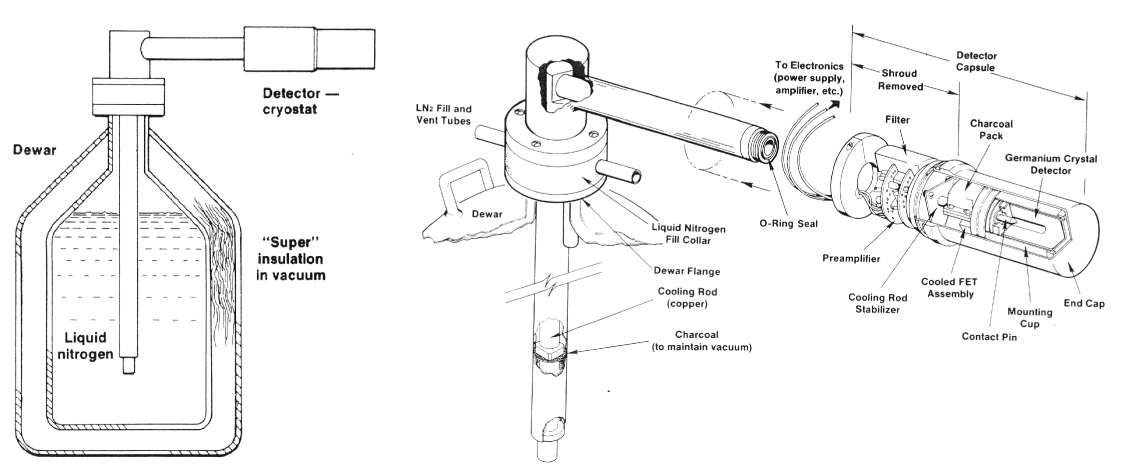
\includegraphics[width=450px, totalheight=450px, keepaspectratio]{DetGes.jpg}
	\caption{Aufbau des gesamten Detektors\\ (Quelle: Praktikumsanleitung)}
	\label{figdetektorges}
\end{figure}


\subsection{Elektronik}

Die durch die Wechselwirkungsmechanismen der $\gamma$ - Quanten im Detektor entstehenden Elektronen geben durch Sto"sprozesse ihre Energie an weitere Elektronen ab, sodass eine Elektronenkaskade im Detektormaterial entsteht. Das dort vorhandene elektrische Feld sorgt daf"ur, dass diese Elektronenkaskade zum n - dotierten Kontakt hin abwandert, wo infolgedessen ein Spannungspuls entsteht. Dieser ist jedoch zu schwach, um direkt messbar zu sein, weshalb er zun"achst verst"arkt werden muss. Die Verst"arkung soll einerseits m"oglichst proportional zur Spannungspulsst"arke erfolgen, gleichzeitig aber keine unerw"unschten statistisch bedingten St"oreffekte oder Rauschen mitverst"arken. Um dies zu erreichen, wird das Signal in mehreren Einzelschritten manipuliert; es durchl"auft zuerst einen Feldeffekttransistor (kurz: FET), der unmittelbar hinter dem Germaniumkristall angebracht ist, um das in Kabeln entstehende Rauschen so gering wie m"oglich zu halten, dann einen Vor- und anschlie"senden Hauptverst"arker, und schlie"slich einen Analog - to - digital - Converter, um das resultierende Signal zuletzt mit einem Vielkanalanalysator untersuchen zu k"onnen.

\begin{figure}[!ht]
	\centering
	\SetFigLayout{1}{1}
	\includegraphics[width=250px, totalheight=250px, keepaspectratio]{mosfet.PNG}
	\caption{Schematischer Aufbau eines MOSFET\\ (Quelle: https://de.wikipedia.org/wiki/Feldeffekttransistor)}
	\label{figmosfet}
\end{figure}

Der FET dient einer ersten Verbesserung der Signalst"arke. Das Funktionsprinzip "ahnelt dem einer Elektronenr"ohre, nur dass der FET Spannungen anstelle von Str"omen verst"arkt. Eine schematische Darstellung am Beispiel des MOSFET - Transistors ist in Abb. \ref{figmosfet} gezeigt. Er besteht aus einem p-dotierten Substrat, in welches zwei n-dotierte Bereiche eingebracht sind. Die im Bild gelb eingef"arbten Bereiche dienen als Isolationsschicht und bestehen oft z.B. aus Siliziumdioxid. Diese Isolationsschichten decken, bis auf kleine L"ucken f"ur die Kontakte an beiden n-Schichten, den gesamten Kristall ab. Am Gate wird oben auf die Isolierschicht eine Aluminiumschicht aufgedampft. Liegt zwischen Source und Gate keine Spannung an, kann kein Strom zwischen Source und Drain flie"sen, da dazu keine freien Ladungstr"ager zwischen den beiden n-Kontakten zur Verf"ugung stehen ("selbstsperrend"). Wird allerdings eine positive Spannung am Gate angelegt, werden Elektronen im p-dotierten Bereich zum Gate hin bewegt (und L"ocher von dort weg) und sammeln sich dort an der Isolierschicht, sodass sich ein Kanal zwischen den n-Kontakten bildet, der Elektronen transportieren kann und es kommt zum Stromfluss zwischen Source und Drain. Die St"arke dieses Stromflusses l"asst sich "uber die am Gate angelegte Spannung steuern.
% Durch ein internes elektrisches Feld erhalten Elektronen, die den FET passieren, zus"atzliche Energie, die zum Einen proportional zu ihrer anf"anglichen Energie und au"serdem proportional zu einer am Transistor angelegten Gate - Spannung ist.  Die an das Gate angelegte Spannung steuert die St"arke des elektrischen Feldes, das sich durch die pn - Kontakte ausbildet. \\
Im n"achsten Schritt durchl"auft das Signal den Vorverst"arker, der es in einen Puls umwandelt, dessen Amplitude proportional zur im Detektor ausgel"osten Ladungsmenge $Q$, antiproportional zur Vorverst"arkerkapazit"at $C$ ist und eine Abfallzeit von ca. 50 $\mu$s hat. Der darauffolgende Hauptverst"arker (kurz: HV) filtert dieses Signal mittels mehrerer Hoch - und Tiefp"asse, die dazu dienen, das Signal weiter zu gl"atten und in eine Semigaussform zu wandeln: Die Tiefp"asse lassen dabei Signalanteile mit niedriger Frequenz weitestgehend ungefiltert hindurch und schw"achen die Anteile mit hoher Frequenz ab, wogegen die Hochp"asse im Gegensatz dazu nur h"ohere Frequenzen ohne Abschw"achung verarbeiten. Beide Elemente bestehen jeweils aus einem Widerstand und einem Kondensator, die in Reihe geschaltet sind; beim Tiefpass folgt auf den Widerstand der Kondensator und "uber dem Kondensator wird die Spannung abgegriffen, beim Hochpass wird die Reihenfolge beider Bauteile vertauscht und auch die Spannung wird stattdessen "uber dem Widerstand abgegriffen (sh. Abb. \ref{youshallnotpass}).

\begin{figure}[!ht]
	\centering
	\SetFigLayout{1}{1}
	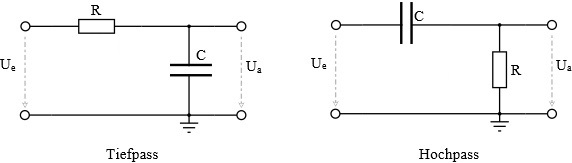
\includegraphics[width=400px, totalheight=400px, keepaspectratio]{hochtief.jpg}
	\caption{Schaltskizze f"ur Tief- und Hochpass\\ (Quelle: https://www.rahner-edu.de/s/cc_images/cache_4775273.jpg?t=1523436560)}
	\label{youshallnotpass}
\end{figure}

Durch das filtern hoher und tiefer Frequenzen verbleibt somit nur ein gewisses Frequenzfenster, das den HV ungefiltert passiert, wodurch die Semigaussform zustande kommt. Die Gr"o"se des Fensters kann "uber die Shaping time Einstellung des HV eingestellt werden; eventuell entstehende Unter- oder "Uberschwinger k"onnen die gemessene Energie beeinflussen und sind mit der Pole-Zero-Einstellung des HV zu beheben.


\subsection{Energieaufl"osung \& Nachweiseffizienz}

Die Aufl"osung des Detektors gibt uns Auskunft dar"uber, wie gro"s die Energiedifferenz zweier Peaks mindestens sein muss, damit wir die Peaks im gemessenen Spektrum noch voneinander unterscheiden k"onnen. Die dabei entscheidende Gr"o"se ist die Halbwertsbreite FWHM (full width at half maximum) des Full - Energy - Peaks, die f"ur eine Gauss - Kurve der Varianz $\sigma$

\begin{equation}
\text{FWHM} = 2\sqrt{2\ln{2}}\cdot \sigma \approx 2.35\sigma
\end{equation}

betr"agt. Die Varianz $\sigma$ h"angt ihrerseits ab von der Anzahl $N$ der im Detektor erzeugten Elektron - Loch Paare\footnote{$N$ ist in Szintillatoren gr"o"ser als in Halbleitern, wodurch sich die schlechtere Energieausfl"osung von Szintillationsdetektoren erkl"art}, welche wiederum von der Energie $E_{\gamma}$ des registrierten $\gamma$ - Quants, sowie vom Fano - Faktor $F$, der den Energieverlust\footnote{Dieser ensteht z.B. dann, wenn ein H"ullenelektron durch Energieaufnahme nur angeregt, das Atom jedoch nicht ionisiert wird, da es dazu zu wenig Energie aufgenommen hat} beim Erzeugen eines solchen Paares beschreibt, abh"angt. Wenn zur Erzeugung eines Elektron - Loch - Paares die Energie $\epsilon$ n"otig ist, ergibt sich eine Mindesthalbwertsbreite von

\begin{equation}
\text{FWHM}_{\text{intrinsisch}} = 2.35\sqrt{\epsilon E_{\gamma} F}
\end{equation}

Dieser intrinsische Anteil der Halbwertsbreite kann nicht unterschritten werden, da er sich aus dem kompletten Detektoraufbau ergibt. Da $\epsilon$ allerdings eine Materialkonstante ist, ergeben sich f"ur verschiedene Detektormaterialien verschiedene intrinsische Halbwertsbreiten. Ge beispielsweise hat einen $\epsilon$ - Wert von ca. 2,8 eV, wogegen Si $\epsilon \approx$ 3,6 eV hat; Ge hat also im Vergleich zu Si die bessere intrinsische Aufl"osung. Zur tats"achlichen FWHM kommen jedoch weitere Anteile, bedingt durch Rauschen, Trapping (also das Einfangen von Ladungen in Gitterfehler - Niveaus) usw hinzu:

\begin{equation}
\text{FWHM}^2 = \text{FWHM}_{\text{intrinsisch}}^2 + \text{FWHM}_{\text{Rauschen}}^2 + \text{FWHM}_{\text{Trapping}}^2 + \dots
\end{equation}

"Uber diese Halbwertsbreite definiert sich schlie"slich die Aufl"osung $R$ des Detektors:

\begin{equation}
R = \frac{\text{FWHM}}{E_{\gamma}}
\end{equation}


Der Detektor kann nur diejenigen $\gamma$ - Quanten erfassen, die von der Quelle in einem bestimmten, kleinen Raumwinkel emittiert werden, in welchem sich der Detektor befindet.
% Diesem Umstand tr"agt die Nachweiseffizienz $\epsilon_{\text{Peak}}$ Rechnung, die wie folgt definiert wird:
Die Information "uber diesen vom Detektor erfassbaren Anteil aller von der Quelle emittierten Photonen fasst man in der geometrischen Effizienz $\epsilon_{\text{Geom.}}$ zusammen; diese Gr"o"se multipliziert mit der intrinsischen Effizienz ergibt die \textit{Nachweiseffizienz} des Detektors, die das Verh"altnis der Anzahl der detektierten $\gamma$ - Quanten zu allen von der Quelle emittierten beschreibt. Um weiteren Eigenschaften des Detektors, wie z.B. materialspezifische Einfl"usse auf die Messung, sowie der Natur der Wechselwirkungen zwischen $\gamma$ - Quanten und Materie Rechnung zu tragen, f"uhrt man au"serdem die \textit{Peakeffizienz} $\epsilon_{\text{Peak}}$ ein, die wie folgt definiert wird:

\begin{equation}
\epsilon_{\text{Peak}} = \frac{\text{detektierte Pulse im Full - Energy - Peak}}{\text{von Quelle emittierte $\gamma$ - Quanten}}
\end{equation}

Diese ber"ucksichtigt im Z"ahler nun nur noch diejenigen Photonen, die ihre gesamte Energie im Detektor abgegeben haben und somit zum Full - Energy - Peak beitragen.
Da das Verh"altnis dieser Anzahl zu allen von der Quelle emittierten Photonen jedoch in der Praxis nur schwierig zu quantisieren ist, bedient man sich zur praktischen Bestimmung der Peakweiseffizienz einer N"aherung mit den freien Parametern $\kappa$, $b$ und $c$:
% Nachweiseffizienz wird unter Anderem durch die Detektorgeometrie und - Abmessungen beeinflusst, durch das Detektormaterial und weitere Faktoren, die schwierig zu quantisieren sind. Daher bedient man sich zur Bestimmung der Nachweiseffizienz einer N"aherung mit den freien Parametern $\kappa$, $b$ und $c$:

\begin{equation}
\epsilon_{\text{Peak}} = \kappa \cdot E_{\gamma}^{b} + c
\end{equation}

Mit zunehmendem $E_{\gamma}$ sinkt infolge der steigenden Anzahl und komplexit"at der Wechselwirkungen des $\gamma$ - Quants mit dem Detektormaterial die Peakeffizienz, da bei zahlreicheren Wechselwirkungen mehr Energie verloren gehen kann. Daher wird $b$ als negativ angesetzt. Im Versuch bestimmen wir die Nachweiseffizienz des Detektors, indem wir diese Funktion als Fitfunktion mit allen drei Parametern als freie Fit - Parameter nutzen.






\section{Versuchsdurchf"uhrung}

Wir erhalten einen Datensatz, der folgende mit dem HPGe - Detektor aufgenommenen $\gamma$ - Spektren enth"alt:

\begin{itemize}
\item{Raumuntergrundmessung ohne Quelle (Messzeit 30 Minuten)}
\item{$^{137}$Cs (Messzeit 450 Sekunden)}
\item{$^{60}$Co (Messzeit 450 Sekunden)}
\item{$^{57}$Co (Messzeit 450 Sekunden)}
\item{$^{22}$Na (Messzeit 450 Sekunden)}
\item{$^{152}$Eu (Messzeit 30 Minuten)}
\end{itemize}

Zwischen s"amtlichen Messungen wurden an der Quelle - Detektor - Geometrie keinerlei Ver"anderungen vorgenommen.
Wir erhalten zudem eine Serie von $\gamma$ - Spektren einer $^{137}$Cs - Quelle mit einer Messzeit von jeweils 2 Minuten. Eine der Messungen wurde mit einem Al - Absorber der Dicke $d = 1$mm zwischen Quelle und Detektor durchgef"uhrt, bei den folgenden 5 Messungen wurden jeweils zus"atzliche Al - Absorber variierender Dicke hinzugef"ugt. Dasselbe wurde anschlie"send mit Pb - Absorbern wiederholt.
Zudem erhalten wir eine Untergrundmessung.

\section{Auswertung}
	\subsection{Pulsformen}
		Da wir diesen Versuch aufgrund der Corona Pandemie nur Online durchf"uhren konnten,
		war uns eine Optimierung der Pole-Zero Einstellung nicht m"oglich. Was h"atte beobachtet werden
		k"onnen w"are: \newline
		Detektiert man ein Ereignis, so nimmt die Amplitude des Spannungspulses nach dem Vorverst"arker
		nahezu linear zu, bis zu einem Maximalwert, nach welchem sie exponentiell abf"allt.
		Die Zeit f"ur den Anstieg dieser Kurve ist dabei die Zeit, in der die Elektron-Loch-Paare
		durch den Halbleiter Kristall zu den Elektroden wandern. Alle Ereignisse bzw. Pulse werden
		somit in dieser Zeit zu einem einzigen Peak aufsummiert. F"ur die Anstiegszeit und Abfallzeit haben
		wir aufgrund der Onlinedurchf"uhrung leider keine Werte. Nach dem Hauptvers"arker h"atte der Impuls eine
		Semi-Gau"sform angenommen, die im rechten Ausl"aufer unter die X-Achse schwingen kann und sich dieser danach eventuell nur langsam ann"ahert; dieser Effekt h"atte sich mithilfe der Pole - Zero - Einstellung korrigieren lassen.
		% bei der die "Anderung der Shaping-Time dazu f"uhren w"urde, dass der rechte
		% Ausl"aufer der Kurve sich nur sehr langsam der x-Achse n"ahert. Dies kann durch die Pole-Zero-Einstellung
		% korrigiert werden.

	\subsection{Eichung und Energieaufl"osung}
		Um die Messdaten n"aher Auswerten zu k"onnen, mussten wir zun"achst die Energieaufl"osung und die Eichung,
		dh. die Korrespondenz von Kanal zu Energie, bestimmen. Dazu werteten wir die Full-Energy Peaks der
		Messungen zu $^{137}$Cs, $^{60}$Co, $^{57}$Co und $^{22}$Na aus und plotteten die Literaturwerte der Energien gegen
		unsere gemessenen Kan"ale.
		Durch einen Fit der Funktion
		\begin{equation}
			E[\text{keV}] = a \cdot \text{Kanalzahl} + b
		\end{equation}

		mit den Werten
		\begin{center}
			\begin{tabular}{|c|c|c|}
				\hline
				Kern & Energy [keV] & Kanalzahl \\
				\hline
				$^{22}$Na & 511 & 2903,565 \\
				& 1275 & 7035,037 \\
				$^{57}$Co & 14,4 & 801,93 \\
				$^{60}$Co & 1173 & 6485,969 \\
						  & 1332 & 7347,992 \\
				$^{137}$Cs & 662 & 3718,27 \\

				\hline
				%\caption{Energieeichung}
			\end{tabular}
		\end{center}
		Ergab sich folgender Fit:
		\begin{figure}[H]
			\centering
			\SetFigLayout{1}{1}
			\includegraphics[width=0.55\textwidth]{Eichung.png}
			%\caption{Schematischer Aufbau eines MOSFET}
			\label{Energieeichung}
			\caption{Energieeichungsfit}
		\end{figure}
		mit der Eichung
		\begin{equation}
			E = 0,185(\pm0,058)\text{keV}\cdot \text{Kanalzahl} - 25,28(\pm30,57)\text{keV}
		\end{equation}
		Damit l"asst sich nun die Energie Der Comptonkanten und R"uckstreupeaks unserer Messung Ermitteln:
		\begin{center}
			\begin{tabular}{|c|c|c|c|c|}
				\hline
				Kern & Ereigniss & Kanal & Energie [keV] & Theoretischer wert\footnote{Dieser ergibt sich gem"a"s Gl. \ref{eqCK} bei Einsetzen der $\gamma$-Energie des zugeh"origen "Ubergangs. Der jeweilige R"uckstreupeak $E_R$ ergibt sich mit der Lage $E_{CK}$ der Compton-Kante aus $E_R = E_{\gamma} - E_{CK}$.} [keV] \\
				\hline
				$^{22}$Na & Comptonkante(High) & 5921 & $1070,11(\pm?)$ & 1062,2 \\
						  & Comptonkante(Low) & 1985 & $341,95(\pm?)$ & 340,0 \\
						  & R"uckstreupeak(High) & ??? & ??? & 212,8 \\
						  & R"uckstreupeak(Low) & 1055 & $169,9(\pm?)$ & 171,0 \\
				$^{57}$Co & Comptonkante(High) & ??? & ??? & 47,5 \\
						  & Comptonkante(Low) & ??? & ??? & 39,5 \\
						  & R"uckstreupeak(High) & ??? & ??? & 89,0 \\
						  & R"uckstreupeak(Low) & ??? & ??? & 82,6 \\
				$^{60}$Co & Comptonkante(High) & 6207 & $1123,02(\pm?)$ & 1118,1 \\
						  & Comptonkante(Low) & 5370 & $968,17(\pm?)$ & 963,4 \\
						  & R"uckstreupeak(High) & 1262 & $208,19(\pm?)$ & 214,4 \\
						  & R"uckstreupeak(Low) & ??? & ??? & 179,8 \\
				$^{137}$Cs& Comptonkante & 2730 & $479,77(\pm?)$ & 477,4 \\
						  & R"uckstreupeak & 1129 & $183,59(\pm?)$ & 184,3 \\
				\hline
				%\caption{Vergleich der Peakpositionen mit Literaturwerten}
			\end{tabular}
		\end{center}



% FOLGENDEN TEXTTEIL NACH ERG�NZUNG DER TABELLE UM FEHLENDE WERTE NEU FORMULIEREN!!!!
% TAUCHEN PEAKS IM GEMESSENEN SPEKTRUM NICHT AUF? WARUM? NIEDRIGE QUELLAKTIVIT�T; HOHE HALBWERTSZEIT DES ZUSTANDS ODER WHATEVER


		Die meisten unserer gemessenen Werte liegen nach der Eichung innerhalb des Fehlerbereichs auf den Literaturwerten. %\footnote{https://www.bmu.de/fileadmin/Daten\_BMU/Download\_PDF/Strahlenschutz/strlsch\_messungen\_gamma\_interf\_bf.pdf}.
		Diese "Ubereinstimmung ist recht "uberraschend, da die Pr"azisen Werte optisch zu bestimmen auf den ersten Blick recht
		ungenau wirkt. Zus"atzlich war bei einigen der Kanten/Peaks nur schwer ein scharfer "Ubergang zu erkennen.
		%Auch f"allt direkt auf, dass einige korrespondierende R"uckstreupeaks und Comptonkanten f"ur $^{57}$Co im SPektrum fehlen, was am eingeschr"ankten Aufnahmebereich unseres Detektors liegt.
		Bei der Messung der Peaks wurde zugleich auch die FWHM (Halbwertsbreite) der Full-Energy Peaks bestimmt,
		wodurch sich der erwartete Zusammenhang von
		\begin{equation}
			\text{FWHM} \propto \sqrt{E_{\gamma}}
		\end{equation}
		"uberpr"ufen lie"s. Tr"agt man die FWHM gegen $\sqrt{E_{\gamma}}$ auf, sollte sich n"aherungsweise eine
		Gerade Zeigen.
		\begin{figure}[H]
			\centering
			\SetFigLayout{1}{1}
			\includegraphics[width=0.55\textwidth]{FWHM.png}
			%\caption{Schematischer Aufbau eines MOSFET}
			\label{fig:Schematischer Aufbau eines MOSFET}
			\caption{Geradenfit f"ur $\sqrt{E_{\gamma}}$ gegen FWHM}
		\end{figure}
		In diesem Plot ist die Halbwertsbreite von $^{22}$Na als Ausrei"ser markiert, da seine Halbwertsbreite von ~2.8keV
		die Qualit"at des Fits stark beeinflussen w"urde.
		
		Die Ursache f"ur diese Abweichung k"onnte in der Zerfallsart des Natriumisotops liegen, denn im Gegensatz zu den anderen im Versuch verwendeten Quellen ist $^{22}$Na ein $\beta^+$ - Strahler. Die beim Zerfall des Isotops emittierten Positronen annihilieren, wie im Theorieteil beschrieben, mit einem Elektron in zwei 511 keV - Photonen, die den zu $^{22}$Na geh"origen 511 keV - Peak erzeugen. Im Schwerpunktsystem der annihilierenden Leptonen werden die Photonen kollinear emittiert, im Laborsystem kann der Emissionswinkel jedoch von 180$^{\circ}$ abweichen, was aufgrund relativistischer Effekte mit einer Dopplerverschiebung der Photonenenergie einhergeht und somit f"ur eine Verbreiterung des zugeh"origen Peaks im Spektrum sorgt. Dies hat eine Abweichung vom erwarteten Zusammenhang FWHM $\propto \sqrt{E_{\gamma}}$ zur Folge.
		
		F"ur die anderen Halbwertsbreiten l"asst sich der lineare
		Zusammenhang jedoch gut best"atigen.
		F"ur die Aufl"osung der Peaks gilt
		\begin{equation}
			A = \frac{\text{FWHM}}{E_{\gamma}} \newline
			\Rightarrow A \propto \frac{\sqrt{E_{\gamma}}}{E_{\gamma}} = \frac{1}{\sqrt{E_{\gamma}}}
		\end{equation}
		\begin{center}
			\begin{tabular}{|c|c|c|c|}
				\hline
				Kern & Energie [keV] & FWHM [keV] & Aufl"osung \\
				\hline
				$^{137}$Cs & 662,63 & 1,46 & 0,22\%  \\
				$^{60}$Co & 1334,13 & 1,992 & 0,15\% \\
						  & 1174,65 & 1,883 & 0,16\% \\
				$^{57}$Co & 123,11 & 1,02 & 0,83\%	\\
				$^{22}$Na & 511,91 & 2,791 & 0,38\% \\
						  & 1276,23 & 1,934 & 0,22\% \\
				\hline
				\label{tabFWHMvsE}
				%\caption{Peakaufl"osungen}
			\end{tabular}
		\end{center}
		Es ist deutlich zu erkennen, das f"ur zunehmende Energien die Aufl"osung steigt.







	\subsection{Bestimmung der Nachweiseffizienz}
		Um die Nachweiseffizienz des Detektors n"aher zu bestimmen, wurde eine Effiziensmessung mit einer $^{152}$Eu-Quelle
		durchgef"uhrt und 30 Minuten lang deren Spektrum aufgezeichnet. Aus dem Resultat haben wir dann die Nettointegrale der
		Full-Energy-Peaks bestimmt und tabelliert. 
		Die Spalte "Normiertes Volumen" gibt die Volumina geteilt durch das Volumen der 1408 keV Linie an:
	
		 $$V_{\text{norm}} = V_{\text{Peak}} / V_{1408\text{keV-Linie}}$$
		 
		 Der zugeh"orige Fehler berechnet sich mittels die allgemeine Fehlerfortpflanzung unabh"angiger Gr"o"sen "uber 
		 
		 $$\Delta V_{\text{norm}} = \sqrt{(\frac{\Delta V}{V_{1408\text{keV-Linie}}})^2 + (\frac{\Delta V_{1408\text{keV-Linie}} \cdot V}{V_{1408\text{keV-Linie}}^2})^2}$$
		 
		 Dieser Wert dividiert durch die Intensit"at des jeweiligen Peaks relativ zur Intensit"at des 1408keV - Peaks, $I_{\text{rel}}$, ergibt einen Wert f"ur die Nachweiseffizienz $\epsilon_{\gamma}$:
		 
		 $$\epsilon_{\gamma} = \frac{V_{\text{norm}}}{I_{\text{rel}}}$$,\\
		 $$\Delta \epsilon_{\gamma} = \sqrt{ (\frac{ \Delta V_{\text{norm}} }{ I_{\text{rel}} })^2 + (\frac{ V_{\text{norm}} \cdot \Delta I_{\text{rel}} }{ I_{\text{rel}}^2 })^2 }$$
		
		
%		Aus diesen bestimmen wir die Effizienz $\epsilon_{\gamma}$, indem wir die
		
		
		
%		kann man durch
		mithilfe dieser Werte k"onnen wir durch
		fitten der Funktion
		\begin{equation}
			\epsilon_{E_{\gamma}} = \kappa \cdot E_{\gamma}^b + c
		\end{equation}
		den Zusammenhang von Energie und Nachweiseffizienz bestimmen.
		
		\begin{center}
			\begin{tabular}{|c|c|c|c|c|}
				\hline
				Energie [keV] & Volumen/Intensit"at & Normiertes Volumen & Relative Intensit"at & $\epsilon_{\gamma}$ \\
				\hline
				121,78 & $(5,87\pm 0,005)E5$ & $13,28\pm 0,064$ & 136,2\% & $9,75\pm 0,05$ \\
				244,69 & $(7,90\pm 0,03)E4$ & $1,79\pm 0,011$ & 35,8\% & $4,99\pm 0,03$ \\
				344,28 & $(2,43\pm 0,005)E5$ & $5,49\pm 0,028$ & 127,5\% & $4,31\pm 0,02$ \\
				367,79 & $(1,03\pm 0,014)E4$ & $0,23\pm 0,003$ & 4,0\% & $5,79\pm 0,08$ \\
				411,12 & $(1,52\pm 0,014)E4$ & $0,34\pm 0,004$ & 10,7\% & $3,22\pm 0,03$ \\
				443,98 & $(1,84\pm 0,015)E4$ & $0,42\pm 0,004$ & 14,8\% & $2,81\pm 0,03$ \\
				688,68 & $(3,47\pm 0,09)E3$ & $0,08\pm 0,002$ & 4,0\% & $1,96\pm 0,05$ \\
				778,90 & $(5,12\pm 0,024)E4$ & $1,16\pm 0,008$ & 61,9\% & $1,87\pm 0,012$ \\
				867,34 & $(1,24\pm 0,013)E4$ & $0,28\pm 0,003$ & 19,9\% & $1,40\pm 0,02$ \\
				964,13 & $(4,26\pm 0,022)E4$ & $0,96\pm 0,007$ & 69,2\% & $1,39\pm 0,01$ \\
				1005,28 & $(6,20\pm 0,1)E3$ & $0,14\pm 0,002$ & 3,1\% & $4,52\pm 0,08$ \\
				1085,91 & $(3,16\pm 0,019)E4$ & $0,71\pm 0,006$ & 46,5\% & $1,54\pm 0,01$ \\
				1089,70 & $(5,33\pm 0,09)E3$ & $0,12\pm 0,002$ & 8,2\% & $1,47\pm 0,03$ \\
				1112,12 & $(3,57\pm 0,02)E4$ & $0,81\pm 0,006$ & 64,9\% & $1,24\pm 0,01$ \\
				1212,95 & $(2,84\pm 0,07)E3$ & $0,06\pm 0,002$ & 6,7\% & $0,96\pm 0,02$ \\
				1299,12 & $(3,98\pm 0,07)E3$ & $0,09\pm 0,002$ & 7,8\% & $1,15\pm 0,02$ \\
				1408,01 & $(4,42\pm 0,021)E4$ & $1,00\pm 0,007$ & 100,0\% & $1\pm 0,007$ \\
				\hline
				%\caption{Nachweiseffizienz am $^{152}$Eu - Spektrum}
			\end{tabular}
		\end{center}
		F"ur diese Auswertung haben wir nur Linien betrachtet, deren relative Intensit"at $\geq 2,5\%$ betrug. Zudem mussten wir zugunsten
		der Fehler die Nachweiseffizienzen f"ur 367,79 keV und 1005,28 keV auslassen.
		\begin{figure}[H]
			\centering
			\SetFigLayout{1}{1}
			\includegraphics[width=0.55\textwidth]{Nachweisseffizienz.png}
			%\caption{Schematischer Aufbau eines MOSFET}
			\label{Nachweiseffizienz}
			\caption{Nachweiseffizienz - Fit}
		\end{figure}
		Der Fit ergab folgende Parameter:
		\begin{equation}
			\epsilon_{\gamma}(E_{\gamma}) = (666,97 \pm 208,77) \cdot E_{\gamma}^{-0,88 \pm 0,07} - (0,15 \pm 0,29)
		\end{equation}
	\subsection{Absorptionskoeffizienten von Al und Pb}
		In diesem Versuchsabschnitt haben wir mithilfe einer $^{137}$Cs Quelle und dem
		Lambert-Beer Gesetz die linearen Absorptionskoeffizienten $\mu_{\text{Al, Pb}}$ von Aluminium und Blei
		bestimmt. Dazu haben wir f"ur verschiedene Dicken des zu betrachtenden Materials
		jeweils 2 Minuten die $\gamma$-Spektren gemessen und daraus die Intensit"at
		der 662keV Linie bestimmt.
		F"ur die Intensit"at der Gammastrahlung gilt:
		\begin{equation}
			I(d) = I_0 \cdot e^{-\mu d} \Rightarrow \frac{I(d)}{I_0} = e^{-\mu d} \Rightarrow \ln{\frac{I(d)}{I_0}} = -\mu d
		\end{equation}
		Durch Auftragen der Logarithmen der normierten Intensit"at erh"alt man mittels linearer Regression den Absorptionskoeffizienten $\mu$.\newline

		\begin{table}[h]
			\begin{minipage}{.5\textwidth}
				\begin{center}
					\begin{tabular}{|c|c|c|}
						\hline
						d [mm] & Intensit"at & $ln(\frac{I}{I_0})$ \\
						\hline
						0 & 10541 & 0 \\
						1 & 10420 & -0,0115454 \\
						5 & 9471 & -0,1070379 \\
						10 & 8739 & -0,187766 \\
						15 & 7849 & -0,2948863 \\
						20 & 6918 & -0,4211457 \\
						30 & 5828 & -0,5925985 \\
						60 & 3286 & -1,1656014 \\
						\hline
					\end{tabular}
				\end{center}
			\end{minipage}
			\begin{minipage}{.5\textwidth}
				\begin{center}
					\begin{tabular}{|c|c|c|}
						\hline
						d [mm] & Intensit"at & $ln(\frac{I}{I_0})$ \\
						\hline
						0 & 10541 & 0 \\
						1.5 & 8919 & -0,1670886 \\
						3 & 7449 & -0,3471926 \\
						6 & 5167 & -0,7129802 \\
						10 & 2246 & -1,5461216 \\
						16 & 1624 & -1,8703802 \\
						\hline
					\end{tabular}
				\end{center}
			\end{minipage}
		\end{table}

		\begin{figure}[H]
			\centering
			 \subfigure[Aluminium]{\includegraphics[width=0.43\textwidth]{AbsorbAl.png}}\quad
			 \subfigure[Blei]{\includegraphics[width=0.43\textwidth]{AbsorbPb.png}}\quad
			 \caption{Absorbtionskoeffizienten Fits}
		 \end{figure}

		Daraus folgt f"ur die Absorptionskoeffizienten aus den Fits:
		$$\mu_{\text{Al}} = 0,0196 \pm 0,00018 \frac{1}{\text{cm}} $$
		$$\mu_{\text{Pb}} = 0,1264 \pm 0,0073 \frac{1}{\text{cm}}$$
		Zudem gilt:
		\begin{equation}
			I = I_0\cdot e^{-\mu d} = I_0\cdot e^{-\overline{n}\sigma}
		\end{equation},
		wobei $d$ die Absorberdicke, $\mu$ die Absorptionskoeffizienten, $\sigma$ den Absorptionsquerschnitt und \newline $\overline{n}=\frac{N_{mol}\cdot N_A}{A}$ die Fl"achenbelegung
		mit der Stoffmenge $N_{mol}$ und der Avogadrokonstanten $N_A$ bezeichnen. \newline
		Daraus ergibt sich f"ur den atomaren Absorptionsquerschnitt:
		\begin{equation}
			\begin{aligned}
				-\mu d = - \overline{n}\sigma \\
				\Leftrightarrow \sigma = \frac{\mu m_{mol}}{N_a\rho}  \\
			\end{aligned}
		\end{equation}
		Daraus folgt f"ur die atomaren Absorbtionsquerschnitte:
		\begin{center}
			\begin{tabular}{|c|c|c|c|c|c|}
				\hline
				Material & Molmasse [g/mol] & Dichte [g/$cm^3$] & $\mu$ [$cm^{-1}$] & $\sigma$ [barn]  & Literaturwerte [barn]\\
				\hline
				Al & 26,98 & 2,7 & $0,196\pm0,00018$& $3,2\pm 0,03$ & 3,345\\
				Pb & 207,2 & 11,34 & $1,264\pm0,0073$ & $37,93 \pm 0,21$ & 37,89\\
				\hline
				\caption{Ermittelte Materialkonstanten \& Literaturwerte\\ Quelle: http://www.nist.gov/pml/data/xcom/index.cfm}
			\end{tabular}
		\end{center}
		Aus der Tabelle geht deutlich hervor, dass Materialien mit h"oherer Ordnungszahl aufgrund ihres h"oheren Absorptionsquerschnitts
		als Absorber besser geeignet sind.






	\subsection{Raumuntergrundmessung}
		Zuletzt folgte eine Messung des Raumhintergrunds ohne jegliche Quelle. Im Folgenden haben wir einmal versucht, die
		wahrscheinlichsten Ursachen der Hintergrundpeaks in Hinsicht auf "Ubereinstimmung der Energien und
		nat"urliches Vorkommen des Elements zu tabbelieren.
		\begin{center}
			\begin{tabular}{|c|c|c|c|c|}
				\hline
				Energie [keV] & M"ogliche Quelle & Theo. Energie [keV] & Alternative Quelle & Theo. Energie [keV]\\
				\hline
				74,58 & $^{228}$Th & 74,4 & Bi K$\alpha 2$ & 74,82 \\
				76,82 & Po $K\alpha 2$ & 76,86 & - & - \\
				238,2 & $^{214}$Pb & 238,4 & $^{231}$Th & 237,8 \\
				241 & $^{235}$U & 240,87 & $^{224}$Ra & 240,99 \\
				249,8 & $^{214}$Pb & 259,22 & - & - \\
				338 & $^{234}$Pa & 338,1 & $^{223}$Ra & 338,28 \\
				351,5 & $^{231}$Pa & 351,51 & $^{211}$Bi & 351,6 \\
				462,4 & $^{214}$Pb & 462 & $^{228}$Ac & 463 \\
				511 & Elek. Annihilation & 511 & $^{214}$Pb & 511 \\
				582,6 & $^{231}$Pa & 583 & $^{214}$Bi & 581,9 \\
				609,1 & $^{231}$Pa & 609 & $^{74}$Ge  & 608,35 \\
				727 & $^{212}$Bi & 727,33 & - & - \\
				767,6 & $^{211}$Pb & 767,51 & $^{214}$Bi & 768,36 \\
				794,3 & $^{235}$U & 794,7 & - & - \\
				860,4 & $^{208}$Tl & 860,56 & - & - \\
				910,5 & $^{210}$Tl & 910 & $^{227}$Th& 910 \\
				963,4 & $^{63}$Cu & 962,06 & $^{214}$Bi & 964,08 \\
				968,6 & $^{228}$Ac & 968,97 & - & - \\
				1120 & $^{214}$Bi & 1120,29 & $^{234}$Pa & 1120,6 \\
				1238 & $^{214}$Bi & 1238,11 & $^{56}$Fe & 1238,28 \\
				1277 & $^{234}$Pa & 1277,7 & $^{228}$Ac & 1276,69 \\
				1460 & K40 & 1460,83 & - & - \\
				1592 & $^{208}$Tl & 1592,5 & - & - \\
				1764 & $^{214}$Bi & 1764,5 & - & - \\
				2104 & $^{208}$Tl & 2103,2 & - & - \\
				2204 & $^{214}$Bi & 2204,21 & - & - \\
				2614 & $^{208}$Tl & 2614,53 & $^{208}$Pb & 2614,53 \\
				\hline
				\caption{Raumuntergrundmessung\\Quelle Literaturwerte: https://inis.iaea.org/collection/NCLCollectionStore/\_Public/29/033/29033666.pdf?r=1}
			\end{tabular}
		\end{center}


\section{Diskussion}



Die Energieeichung lie"s sich problemlos durchf"uhren und die meisten der damit von uns ermittelten Werte liegen, im Rahmen der Fehler, bei den Literaturwerten. Es sind jedoch auch einige nennenswerte Ausrei"ser aufgetreten, viele davon im $^{22}$Na - Spektrum, wie z.B. beim Auftragen der Peakenergien $\sqrt{E_{\gamma}}$ gegen ihre Halbwertsbreiten (sh. Abb. \ref{figFWHMvsE} \& Tab. \ref{tabFWHMvsE}). Die Ursache f"ur diese Abweichungen k"onnte in der Zerfallsart des Natriumisotops liegen, denn im Gegensatz zu den anderen im Versuch verwendeten Quellen ist $^{22}$Na ein $\beta^+$ - Strahler. Die beim Zerfall des Isotops emittierten Positronen zerfallen, wie im Theorieteil beschrieben, "uber Annihilation mit einem Elektron in zwei 511 keV - Photonen, die den zu $^{22}$Na geh"origen 511 keV - Peak erzeugen. Im Schwerpunktsystem der annihilierenden Leptonen werden die Photonen kollinear emittiert, im Laborsystem kann der Emissionswinkel jedoch von 180$^{\circ}$ abweichen, was aufgrund relativistischer Effekte mit einer Dopplerverschiebung der Photonenenergie einhergeht und somit f"ur eine Verbreiterung des zugeh"origen Peaks im Spektrum sorgt. Dies hat eine Abweichung vom erwarteten Zusammenhang FWHM $\propto \sqrt{E_{\gamma}}$ zur Folge.\\
Im $^{152}$Eu - Spektrum lie"sen sich nicht alle in der Versuchsanleitung aufgef"uhrten Peaks identifizieren. Es handelt sich um eine Quelle mit vergleichsweise niedriger Aktivit"at (28,5 kBq\footnote{Quelle: Versuchsanleitung}), sodass der Raumuntergrund die Messung so stark "uberlagert, dass nicht alle erwarteten Peaks klar als solche erkennbar waren.\\
Bei der Analyse des Raumuntergrundes selbst war es nicht immer m"oglich, eine eindeutige Quelle f"ur die beobachteten $\gamma$ - Energien zu identifizieren, was aufgrund der regionalen Unterschiede und des Reichtums nat"urlich auftretender Radionuklide wenig verwunderlich ist. Viele Linien in den Spektren verschiedener nat"urlich auftretender Radionuklide liegen so dicht beeinander, dass eine klare Linientrennung und -zuordnung bei der gegebenen Detektoraufl"osung nicht m"oglich ist.




\begin{thebibliography}{}
\bibitem[1]{lit1} Versuchsanleitung
\bibitem[2]{lit2} https://www.bmu.de/fileadmin/Daten\_BMU/Download\_PDF/Strahlenschutz/\\strlsch\_messungen\_gamma\_interf\_bf.pdf
\bibitem[3]{lit3} http://www.nist.gov/pml/data/xcom/index.cfm
\bibitem[4]{lit4} https://inis.iaea.org/collection/NCLCollectionStore/\_Public/29/033/29033666.pdf?r=1
\bibitem[5]{lit5} Knoll, Glenn F.:\newline \textit{Radiation detection and Measurement}\newline Wiley, 2000
\end{thebibliography}


\end{document}